\documentclass{beamer}
\usepackage[utf8]{inputenc}
\usepackage[T1]{fontenc}

\title{Project Report}
\subtitle{\textit{Week 5}}
\date[]{2024/2025}
\author[Fritz]{Fritz Adelbertus Sitindaon}

\usetheme{Warsaw}
\setbeamertemplate{footline}[frame number]
% ===== Setup Font =====
\usepackage[sfdefault,lf]{carlito}
\usepackage[T1]{fontenc}
\renewcommand*\oldstylenums[1]{\carlitoOsF #1}

% ==== Import Math Packages =====
\usepackage{amsmath, amssymb, amsthm}
\usepackage{mathtools}

% ==== There required =====
\usepackage[dvipsnames]{xcolor}
\usepackage[most]{tcolorbox}
\def\wallpaper{wallpaper.jpg}

\def\R{\mathbb{R}}
\def\P{\mathbb{P}}
\def\N{\mathbb{N}}
\def\O{\mathbb{O}}


\def\nX{\mathcal{X}}
\def\nY{\mathcal{Y}}
\def\nT{\mathcal{T}}
\def\nU{\mathcal{U}}
\def\nB{\mathcal{B}}
\def\nS{\mathcal{S}}
\def\nP{\mathcal{P}}
\def\nA{\mathcal{A}}
\def\nF{\mathcal{F}}
\newcommand{\comp}[1]{\overline{#1}} 

\DeclarePairedDelimiter\abs{\lvert}{\rvert}
\DeclarePairedDelimiter\floor{\lfloor}{\rfloor}
\DeclarePairedDelimiter\cic{[ }{] }
\DeclarePairedDelimiter\oic{( }{] }
\DeclarePairedDelimiter\cio{[ }{) }
\DeclarePairedDelimiter\oio{( }{) }
\DeclarePairedDelimiter\set{\{ }{\} }
\DeclarePairedDelimiter\brk{(}{)}
\DeclarePairedDelimiter\seq{\langle}{\rangle}

\begin{document}

\begin{frame}
\titlepage
\end{frame}

\begin{frame}{Next Week Target}
    Target for Next Week:
    \begin{enumerate}
        \item Finishing the output to precisely mimic the output in COMCOT Fortran (\textcolor{green}{done})
        \item Adding comments and reorienting the order of functions in code for  
        better readability and easier though process when reading (\textcolor{green}{done})
        \item Creating a documentation/README (\textcolor{orange}{not yet..})
    \end{enumerate}
\end{frame}

\begin{frame}{Output Comparison}
    Input: 100x100 grid\\
    Fortran - Haskell
    \begin{center}
        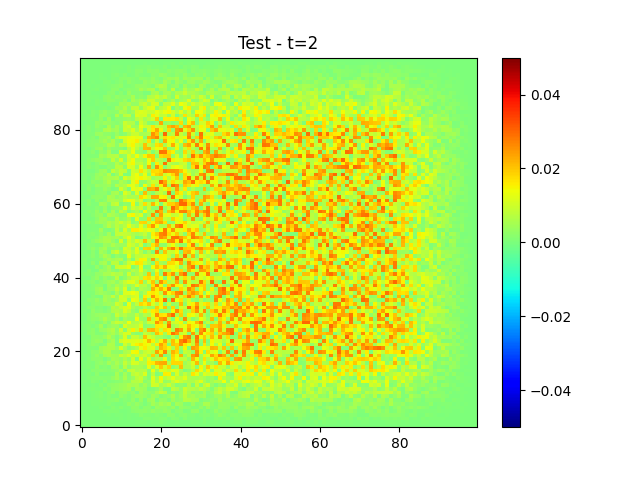
\includegraphics[scale=0.32]{figure/frame_2.png}
        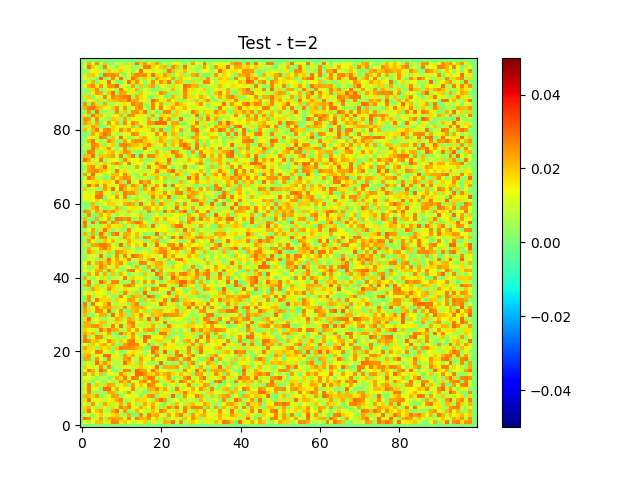
\includegraphics[scale=0.32]{figure/frame_2_2.png}
    \end{center}
\end{frame}

\begin{frame}{Output Comparison}
    Input: 100x100 grid\\
    Fortran - Haskell
    \begin{center}
        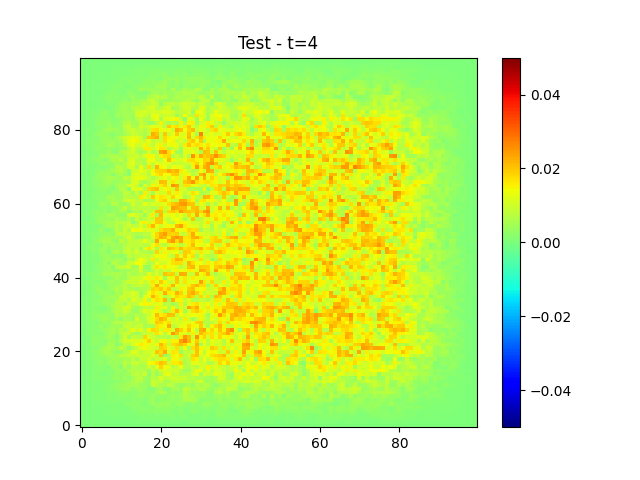
\includegraphics[scale=0.32]{figure/frame_4.png}
        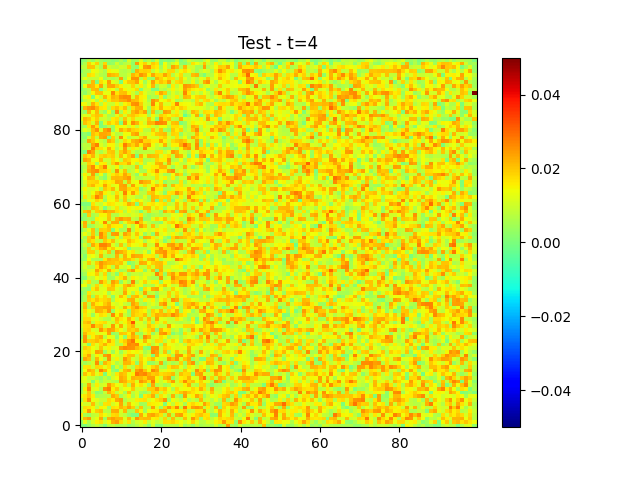
\includegraphics[scale=0.32]{figure/frame_2_4.png}
    \end{center}
\end{frame}

\begin{frame}{Output Comparison}
    Input: 100x100 grid\\
    Fortran - Haskell
    \begin{center}
        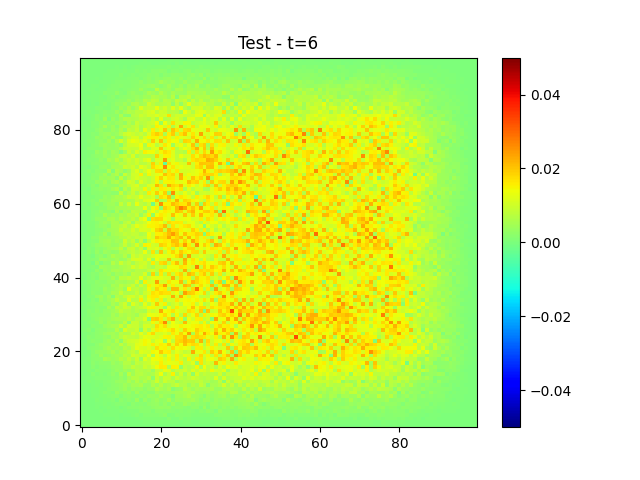
\includegraphics[scale=0.32]{figure/frame_6.png}
        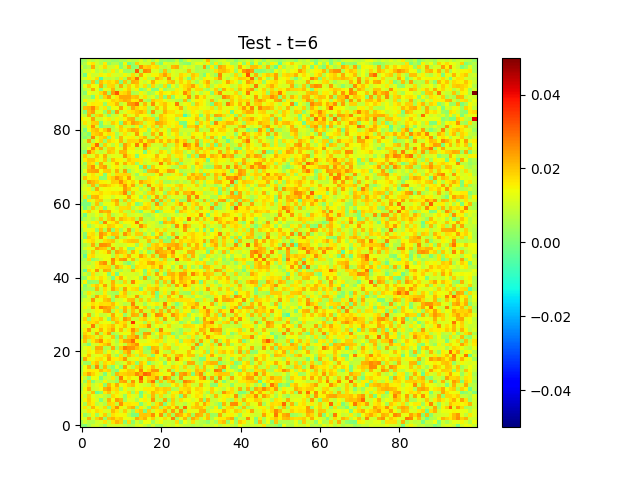
\includegraphics[scale=0.32]{figure/frame_2_6.png}
    \end{center}
\end{frame}

\begin{frame}{Output Comparison}
    Input: 100x100 grid\\
    Fortran - Haskell
    \begin{center}
        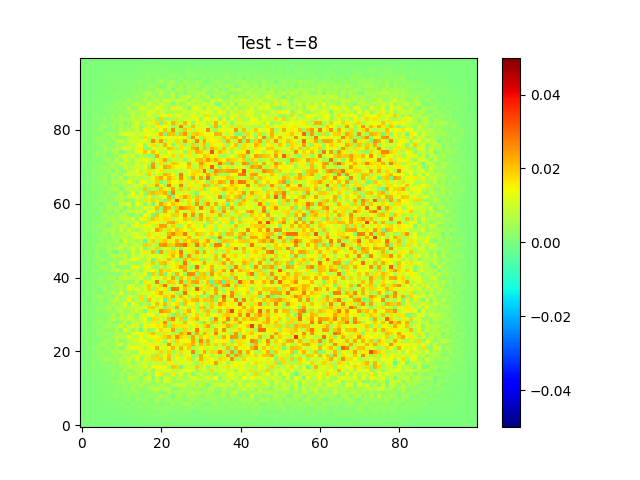
\includegraphics[scale=0.32]{figure/frame_8.png}
        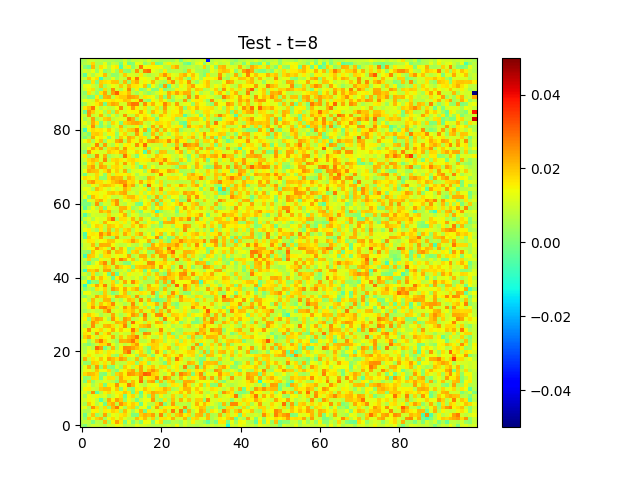
\includegraphics[scale=0.32]{figure/frame_2_8.png}
    \end{center}
\end{frame}

\begin{frame}{Output Comparison}
    Input: 100x100 grid\\
    Fortran - Haskell
    \begin{center}
        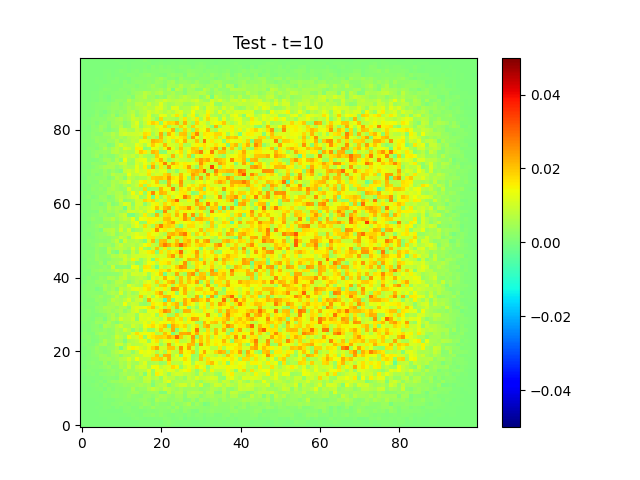
\includegraphics[scale=0.32]{figure/frame_10.png}
        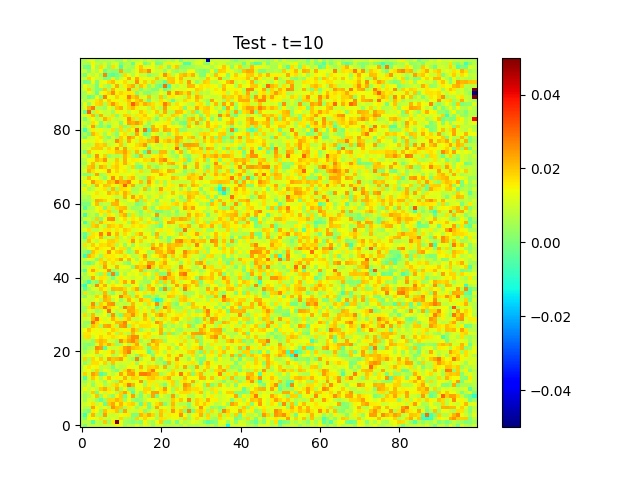
\includegraphics[scale=0.32]{figure/frame_2_10.png}
    \end{center}
\end{frame}

\begin{frame}{Output Comparison}
    \begin{enumerate}
        \item Hasil di Haskell berbeda dengan Fortran dengan toleransi $10^{-3}$.
        \item Hasil di Haskell tetap konsisten terhadap perilaku gelombang tsunami.
    \end{enumerate}
\end{frame}


\begin{frame}{Next Week Target}
    Target for Next Week:
    \begin{enumerate}
        \item Start finishing all project output requirements ()
    \end{enumerate}
\end{frame}

\end{document}